% Preamble
\documentclass[a4paper, 10pt]{report}
\usepackage{geometry}
\geometry{a4paper, top=2cm, bottom=2cm, left=2cm, right=2cm, heightrounded, bindingoffset=5mm}
\bibliographystyle{ACM-Reference-Format}
\usepackage[T1]{fontenc}
\usepackage[utf8]{inputenc}
\usepackage[italian]{babel}
\usepackage{lipsum}
\usepackage{url}
\usepackage{array}
\usepackage{color}
\usepackage{colortbl}
\usepackage{adjustbox}
\usepackage[dvipsnames]{xcolor}
\usepackage{graphicx}
\usepackage[colorlinks = true,
    linkcolor = darkgray,
    urlcolor  = darkgray,
    citecolor = white,
    anchorcolor = darkgray]{hyperref}

\makeatletter
\def\@makechapterhead#1{%
    \vspace*{1\p@}%
    {\parindent \z@ \raggedright
    \normalfont
    \interlinepenalty\@M
    \Huge \bfseries\thechapter\space  #1\par\nobreak
    \vskip 20\p@
    }}
\makeatother

% Document
\begin{document}

    \title{
\includegraphics[width=10cm]{logo.JPEG} \\ \textcolor{Goldenrod}{\textbf{Università degli Studi di Salerno}} \\
    Documentazione progetto\\
    \begin{small}
        Fondamenti di Intelligenza Artificiale \\ a.a. 2022/2023 prof. Fabio Palomba
    \end{small}}
    \author{
        \begin{tabular}{p{5cm}l}
            \textit{Autore} & \textit{Matricola}\\
            \hline
            Costante Luigina & 0512110457\\
            Lo Conte Simona & 0512110922\\
            Napolillo Marta & 0512109836 \\
        \end{tabular}
    }
    \date{}
    \maketitle

    \tableofcontents

    \chapter{Introduzione}\label{ch:introduzione}

        Con l'avvento del digitale è in costante crescita il numero di persone - di ogni fascia di età - che scelgono
        di guardare un film nel proprio tempo libero. Di conseguenza, aumenta la voglia di scoprire sempre nuovi contenuti
        in base alle proprie preferenze e rimanere costantemente aggiornati sulle ultime novità. La maggior parte degli utenti,
        però, è spesso indecisa su quale film scegliere e passa gran parte del tempo a navigare tra i contenuti disponibili.
        A tal proposito \textit{iLike}, oltre a realizzare una piattaforma unificata che consente di recensire contenuti, offre
        la possibilità di interagire con un Conversational Agent, il cui ruolo principale è fornire all'utente indicazioni circa possibili
        film da vedere, sulla base delle sue preferenze.
        Il Conversational Agent è di fondamentale importanza poichè permette agli utenti di ottenere consigli attraverso una
        conversazione simil-umana.


    \chapter{Business Understanding}\label{ch:business-understanding}

        \section{Obiettivi di business}\label{sec:obiettivi-di-business}

            L'obiettivo principale di \textit{iLike} è la realizzazione di un Conversational Agent, che permetterà all'utente di
            interagirvi per richiedere consigli su nuovi film da guardare. Lo scopo è quello di consentire anche agli utenti più indecisi
            di ricevere consigli personalizzati su film che potrebbero essere di interesse personale.
            Tutto ciò sarà possibile analizzando le diverse liste degli iscritti, nelle quali quest'ultimi potranno decidere di inserire contenuti
            diversi in base alle preferenze personali.

        \section{PEAS}\label{sec:peas}

            Specifica PEAS dell'ambiente.\\
            \begin{center}
                \begin{tabular}{|>{\columncolor{Goldenrod}}c|p{8cm}|}
                    \hline
                    \textbf{Performance} & Capacità dell’agente di suggerire all’utente film che rispecchiano i suoi gusti. \\
                    \hline
                    \textbf{Environment} & L’ambiente in cui l’agente opera è rappresentato da iLike, un’applicazione in cui gli
                    utenti possono scrivere recensioni ed esprimere preferenze sui contenuti che si trovano all’interno di essa.\\
                    \hline
                    \textbf{Actuators} & Risposta del Conversational Agent.\\
                    \hline
                    \textbf{Sensors} & Utterances (messaggi in linguaggio naturale dati in input al CA da un utente umano).\\
                    \hline
                \end{tabular}
            \end{center}


        \section{Proprietà dell'ambiente}\label{sec:proprieta-dell'ambiente}
            L’ambiente possiede le seguenti proprietà:
            \begin{itemize}
                \item \textbf{Completamente osservabile}: l’agente ha accesso all’elenco dei contenuti presenti nell’applicazione
                e alle preferenze degli utenti in qualsiasi momento;
                \item \textbf{Stocastico}: lo stato dell’ambiente varia indipendentemente dall’azione intrapresa dall’agente;
                \item \textbf{Sequenziale}: le decisioni prese dall’agente dipendono dalle azioni passate dell’utente;
                \item \textbf{Statico}: nel momento in cui l’agente sta elaborando la sua decisione l’utente non può modificare
                le sue preferenze;
                \item \textbf{Discreto}: i suggerimenti dati dall’agente dipendono dalla combinazione di contenuti preferiti di cui
                l’utente dispone o da un genere stabilito ed esistono un numero limitato di possibili combinazioni;
                \item \textbf{Singolo-agente}: esiste un unico agente che opera nell’ambiente.
            \end{itemize}

        \section{Analisi del problema}\label{sec:analisi-del-problema}

            Il problema che l'agente intelligente dovrà risolvere consiste nel suggerire film da vedere in base ai contenuti
            presenti nei dataset dell'applicazione e soprattutto in merito alle preferenze espresse dagli utenti (in base ai
            contenuti della lista preferiti dell'iscritto).\\
            Il problema in esame può essere risolto con un algoritmo di apprendimento, in quanto consiste nel migliorare l'esecuzione
            di un task (T= fornire suggerimenti personalizzati) rispetto ad una misura di prestazione (P= numero di suggerimenti accettati
            dall'utente) e sulla base dell'esperienza (E= database di contenuti). Inoltre l'algoritmo di apprendimento
            in questione è di tipo non supervisionato in quanto l'agente dovrà essere capace di apprendere il valore reale della
            variabile dipendente sulla base delle conoscenze di cui dispone.
            Nello specifico il problema in esame può essere risolto tramite l'utilizzo di un algoritmo di clustering. Una volta che l'utente
            ha espresso le sue preferenze riguardanti contenuti presenti nell'applicazione, l'algoritmo creerà, in base ad una misura di similarità
            (definita in fase di modelling), dei cluster contenenti film che hanno un certo grado di omogeneità. Procederà quindi a consigliarne nuovi
            in base alla clusterizzazione effettuata.

            I suggerimenti verranno dati solo qualora l'utente ne faccia richiesta ed il tutto avviene in maniera automatica tramite l'utilizzo
            di un Conversational Agent. L'iscritto potrà interagire con quest'ultimo ogni qualvolta lo ritenga opportuno mediante un apposito
            pulsante presente nel footer delle varie activity dell'applicazione. Una volta premuto tale pulsante l'utente potrà scrivere messaggi
            in base ai quali riceverà una risposta opportuna. Nel momento in cui richiederà un consiglio per un film, il Conversational Agent
            chiederà l'algoritmo che si vuole utilizzare e successivamente provvederà ad analizzare l'insieme di cluster di cui si dispone e
            "calcolare" la relativa risposta.

            Si è ritenuto non opportuno utilizzare un algoritmo di classificazione in quanto non disponiamo di un'insieme di osservazioni per cui
            la variabile target è nota, di conseguenza non sarebbe possibile stimare il valore di una nuova variabile categorica.
            Un'analoga considerazione è stata fatta in merito all'utilizzo di un algoritmo di regressione, anche se in questo caso occorreva
            stimare il valore di una variabile numerica.


    \chapter{Data Understanding}\label{ch:data-understanding}

        \section{Acquisizione dei dataset}\label{sec:acquisizione-dei-dataset}
            Durante la scelta dai dati da fornire al machine learning le possibili scelte da seguire erano sostanzialmente due:
            \begin{itemize}
                \item Creare un dataset contenente gli utenti di iLike ed analizzare il loro comportamento, al fine di creare
                cluster di utenti i quali hanno preferenze similari;
                \item Cercare dataset con le informazioni relative ai film e creare cluster di film.
            \end{itemize}\\

            I pro e i contro delle alternative sopra elencate sono:
            \begin{itemize}
                \item La disponibilità di dati era maggiore nei dataset già esistenti;
                \item Ogni utente ha gusti differenti, quindi la similarità tra utenti, rappresentata come il numero di contenuti uguali
                appartente alle proprie liste, può non essere sempre veritera;
                \item Individuare dataset con un numero ottimale di istanze e le giuste informazioni sui film richiede
                un'accurata analisi.
            \end{itemize}
            Al seguito di un trade-off tra le due alternative abbiamo preferito utilizzare dataset già esistenti relativi ai film,
            poichè la disponibilità di dati e la giusta similarità di elementi in un cluster agevola le prestazioni dell'algoritmo
            di machine learning.

        \section{Analisi dei dataset}\label{sec:analisi-dei-dataset}
            Il dataset utilizzato riguardo i \href{https://www.kaggle.com/datasets/stefanoleone992/filmtv-movies-dataset?resource=download}{\underline{Film}}
            è reperibile sulla piattaforma Kaggle.


    \chapter{Data Preparation}\label{ch:data-preparation}
        In fase di Data Understanding abbiamo scelto l'utilizzo di un dataset già esistente, quindi è opportuno effettuare Data Preparation.
        Lo scopo di questa fase è preparare i dati al fine di passarli correttamente all'algoritmo di Machine Learning.

        \section{Data Cleaning}\label{sec:data-cleaning}
            Lo scopo del Data Cleaning è gestire dati rumorosi e/o nulli.
            A tal proposito, è stata effettuata inizialmente un'analisi dei dati al fine di evidenziare dati rumorosi.
            Si è notato che le colonne 'voto\_medio' e 'voti\_totali' rispecchiano esattamente la media e la somma delle colonne
            'voto\_critica' e 'voto\_pubblico'. Dunque abbiamo deciso di eliminare le colonne 'voto\_critica' e 'voto\_pubblico' e
            non eliminare le colonne 'voto\_medio' e 'voti\_totali', rimandando tale scelta nel Feature Selection, per valutare
            quale delle due ha una maggiore correlazione tra le altre variabili.

            In seguito è riportata una tabella contenente il nome della colonna, il numero di elementi mancanti e la scelta di
            Data Imputation effettuata.\\

            \begin{center}
                \begin{tabular}{ |c|c|c| }
                    \hline \rowcolor{Goldenrod} Nome Colonne & Numero Elementi & Scelta Data Imputation \\
                    \hline genere & 95 & Eliminazione Riga \\
                    \hline paese & 11 & Eliminazione Riga \\
                    \hline registi & 33 & Eliminazione Riga \\
                    \hline attori & 2.027 & Eliminazione Colonna \\
                    \hline descrizione & 1.449 & Eliminazione Riga \\
                    \hline note & 21.628 & Eliminazione Colonna \\
                    \hline
                \end{tabular}
                \\
            \end{center}


            Le scelte sopra riportate sono state effettuate per evitare di eliminare un eccessivo numero di righe.
            Si fa eccezione per la colonna descrizione in quanto tale colonna è necessaria all'interno dell'applicazione
            iLike, per altre funzionalità non riguardanti il modulo di Intelligenza Artificiale.

        \section{Feature Scaling}\label{sec:feature-scaling}
            Lo scopo del Feature Scaling è normalizzare i valori numerici del dataset, portandoli tutti nello stesso range.
            I grafici box plot sottoriportati confrontano i valori iniziali e i valori ottenuti prima con la tecnica del
            Min-Max Normalizzation e in seguito con lo Z-Score Normalizzation.

            \begin{center}
                % prima del Feature Scaling
                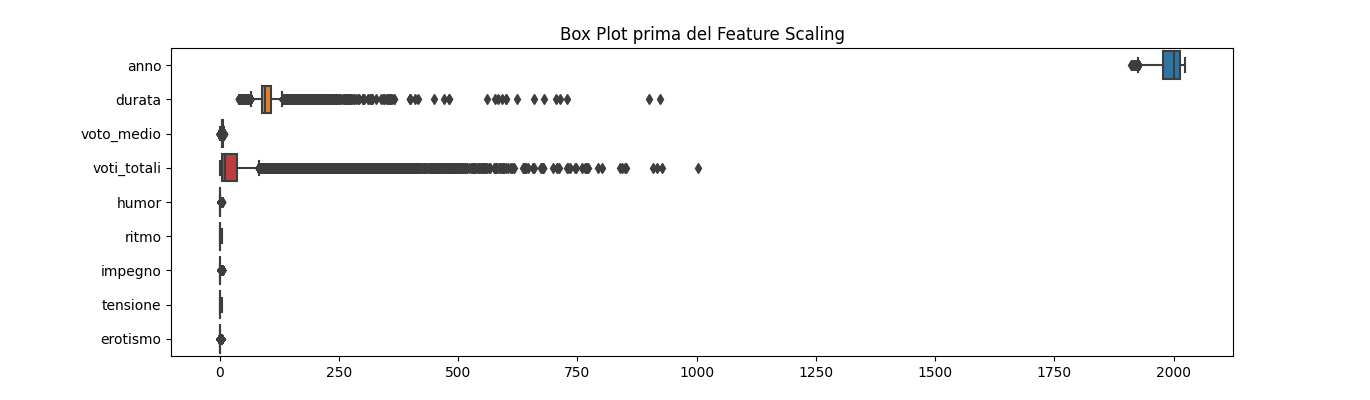
\includegraphics[width=13cm, height=5cm]{dataPreparation/noScaling.png}\\
                % con Min-Max normalizzation
                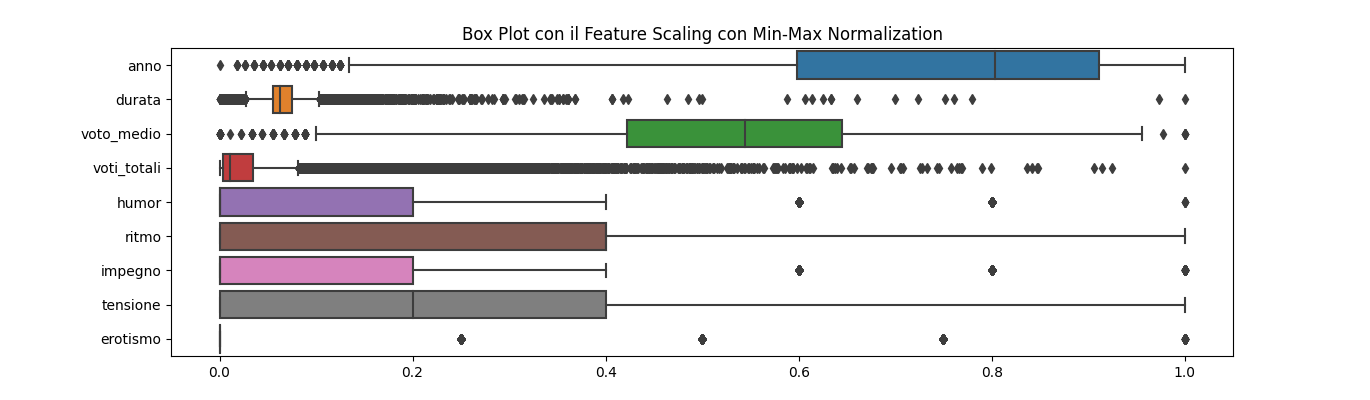
\includegraphics[width=13cm, height=5cm]{dataPreparation/minMax.png}\\
                % con Z-Score Normalizzation
                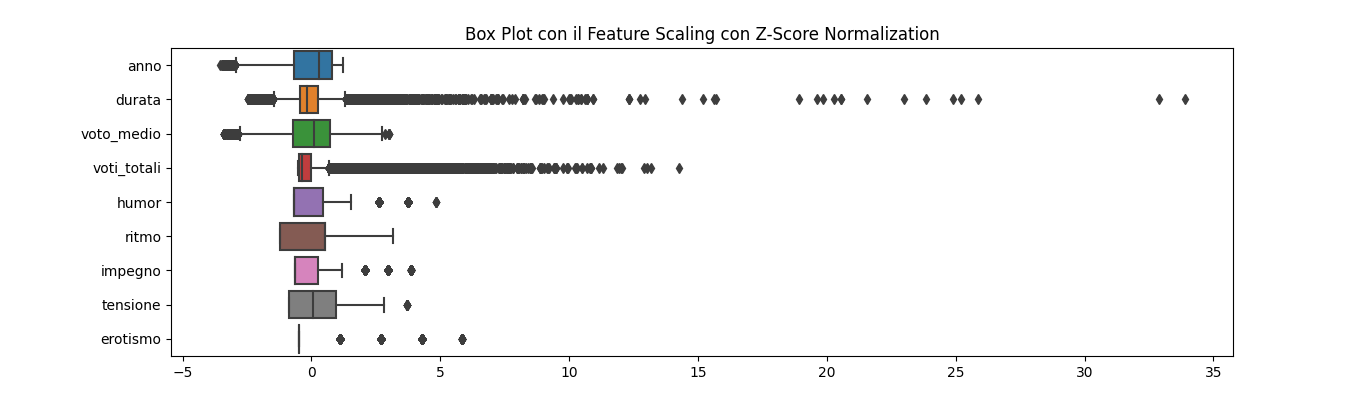
\includegraphics[width=13cm, height=5cm]{dataPreparation/zScore.png}\\
            \end{center}

            \\Come evidenziato nei grafici, la tecnica dello Z-Score Normalizzation è meno tendente ai valori estremi.
            Dunque, abbiamo preferito tale tecnica al fine di effettuare una corretta normalizzazione dei dati.

        \section{Feature Selection}\label{sec:feature-selection}
            Lo scopo del Feature Selection è selezionare le caratteristiche più correlate al problema in esame.
            Le feature dal nostro dataset sono di tipo string o int. Le feature di tipo string rappresentano
            solo informazioni descrittive dei film. Per tal motivo, le feature individuate sono di tipo int.
            In questa fase, le tecniche utilizzate sono:
            \begin{itemize}
                \item Eliminazione di feature con bassa varianza. Con questa tecnica vengono eliminate le feature
                con varianza uguale a zero. Nel nostro caso, nessuna feature a noi diponibile ha varianza uguale a zero;
                \item Eliminazione univariata di feature. Con questa tecnica si analizzano le correlazioni tra le variabili.
                Il grafico sotto riportato offre un'analisi riassuntiva delle correlazioni con le variabili.
                \begin{center}
                    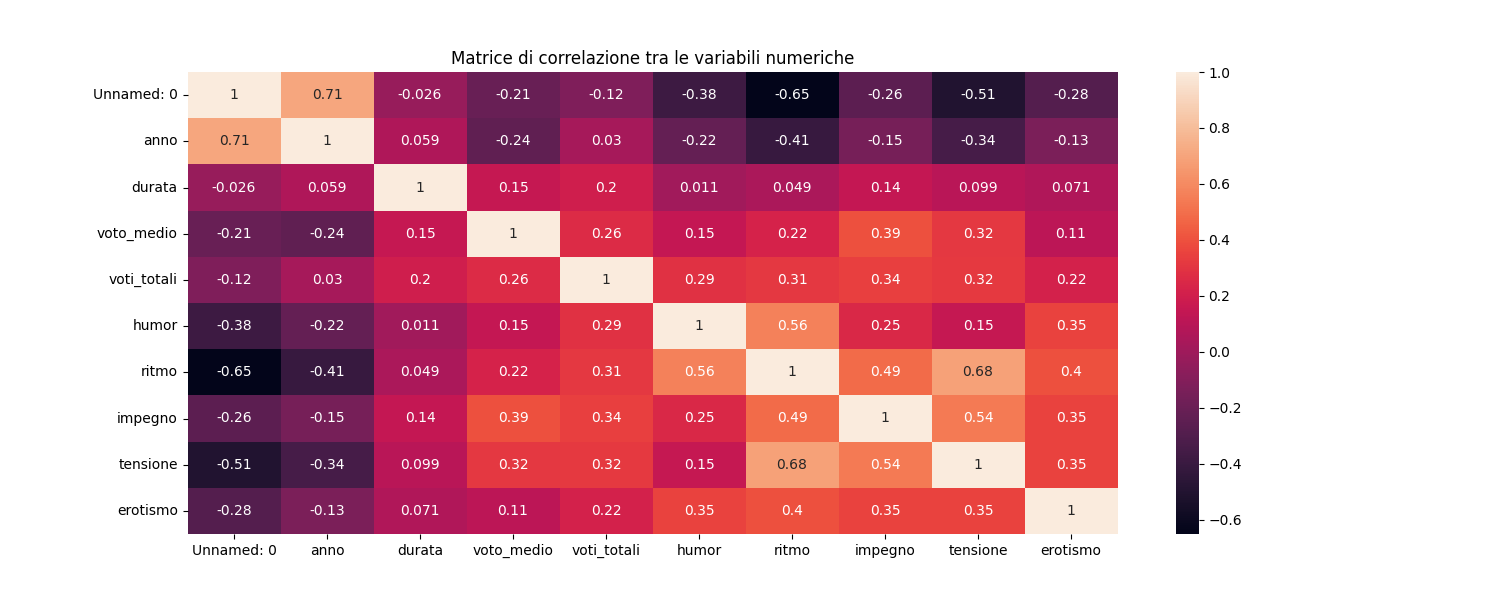
\includegraphics[width=13cm, height=7cm]{dataPreparation/Matrice di Correlazione.png}\\
                \end{center}
                Come si può notare la feature 'anno' è inversamente correlata con quasi tutte le variabili, e la variabile
                'voto\_medio' ha meno correlazione tra le variabili rispetto a 'voto\_totale'.
                Dunque abbiamo eliminato le feature 'anno' e 'voto\_medio'.
            \end{itemize}

        \section{Data Balancing}\label{sec:data-balancing}
            Lo scopo del Data Balancing è bilanciare i dati, al fine di avere lo stesso numero di istanze in tutte le classi.
            Nel nosto dataset le classi possono essere rappresentate dalla feature 'genere', ma avendo optato in fase di
            Business Understanding per un algoritmo di apprendimento non supervisionato, tale bilanciamento non è necessario
            in fase di Data Preparation.


    \chapter{Modeling}\label{ch:modeling}

        \section{Scelta dell'algoritmo da utilizzare}\label{sec:scelta-dell'algoritmo-da-utilizzare}
            Esiste un gran numero di algoritmi di clustering, pertanto bisogna effettuare una scelta dell'algoritmo da considerare
            per effettuare il clustering tra gli elementi.
            Prima di effettuare la scelta dell'algoritmo da utilizzare abbiamo fatto un confronto tra due algoritmi di clustering molto
            usati, ossia il K-Means e il DBScan.

            \subsection{K-Means}
                Per quanto riguarda l'algoritmo di clustering K-Means, questo viene realizzato tramite la funzione KMeans()
                della libreria sklearn.cluster.
                Tale funzione permette di definire alcuni parametri di input, pertanto abbiamo valutato l'algoritmo di K-Means
                con diversi valori per due di questi parametri.

                Per il parametro che permette di definire il metodo per l'inizializzazione abbiamo valutato due opzioni:
                    \begin{itemize}
                        \item random, che sceglie n cluster di osservazioni (righe) a caso dai dati per i centroidi iniziali
                        \item k-means++, che garantisce un'inizializzazione più intelligente dei centroidi e migliora la qualità del clustering
                    \end{itemize}

                Dopo aver valutato i due metodi di inizializzazione sul nostro dataset, abbiamo scelto il metodo k-means++, in quanto più adatto
                a dividere il nostro dataset in cluster distinti.

                Per quanto riguarda il parametro che specifica l'algoritmo che utilizza il K-Means abbiamo valutato le seguenti opzioni:
                \begin{itemize}
                    \item llyod, che è quello utilizzato di default
                    \item elkan, che usa la disuguaglianza triangolare
                \end{itemize}

                A seguito di un confronto abbiamo preferito utilizzare l'algoritmo di elkan, in quanto il numero di iterazioni effettuate per arrivare ad ottenere
                i cluster era nettamente minore al numero di iterazioni effettuate scegliendo l'algoritmo di llyod.

                Il grafico riportato sotto mostra la divisione del dataset in cluster, effettuata utilizzando l'algoritmo di K-Means.

                \begin{center}
                    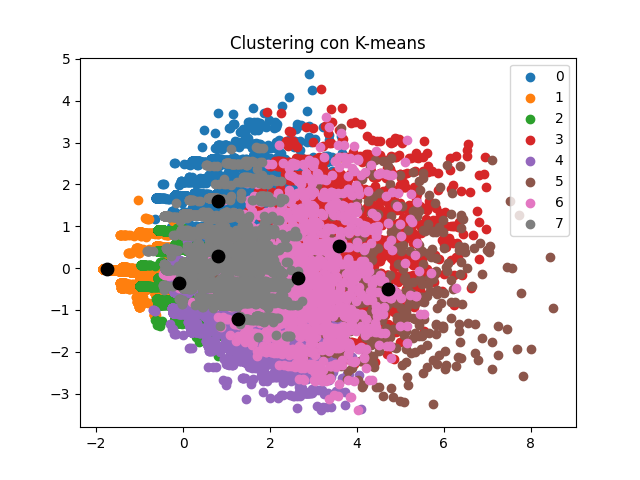
\includegraphics[width=8cm]{modelling/ClusterK-Means.png}\\
                \end{center}

            \subsection{DBScan}
                L'algoritmo di clustering DBScan viene realizzato tramite la funzione DBSCAN() della libreria sklearn.cluster.
                Anche questa funzione permette di definire alcuni parametri di input, che sono:
                \begin{itemize}
                    \item eps, che definisce un intorno circolare di ciascun punto dai suoi vicini
                    \item min samples, che stabilisce il numero minimo di punti per considerare un intorno di un punto denso
                \end{itemize}

                La scelta dei valori effettuata è stata eps=1 e min samples=5.

                Di seguito è riportato il clustering ottenuto con DBScan con i valori dei parametri definiti sopra.

                \begin{center}
                    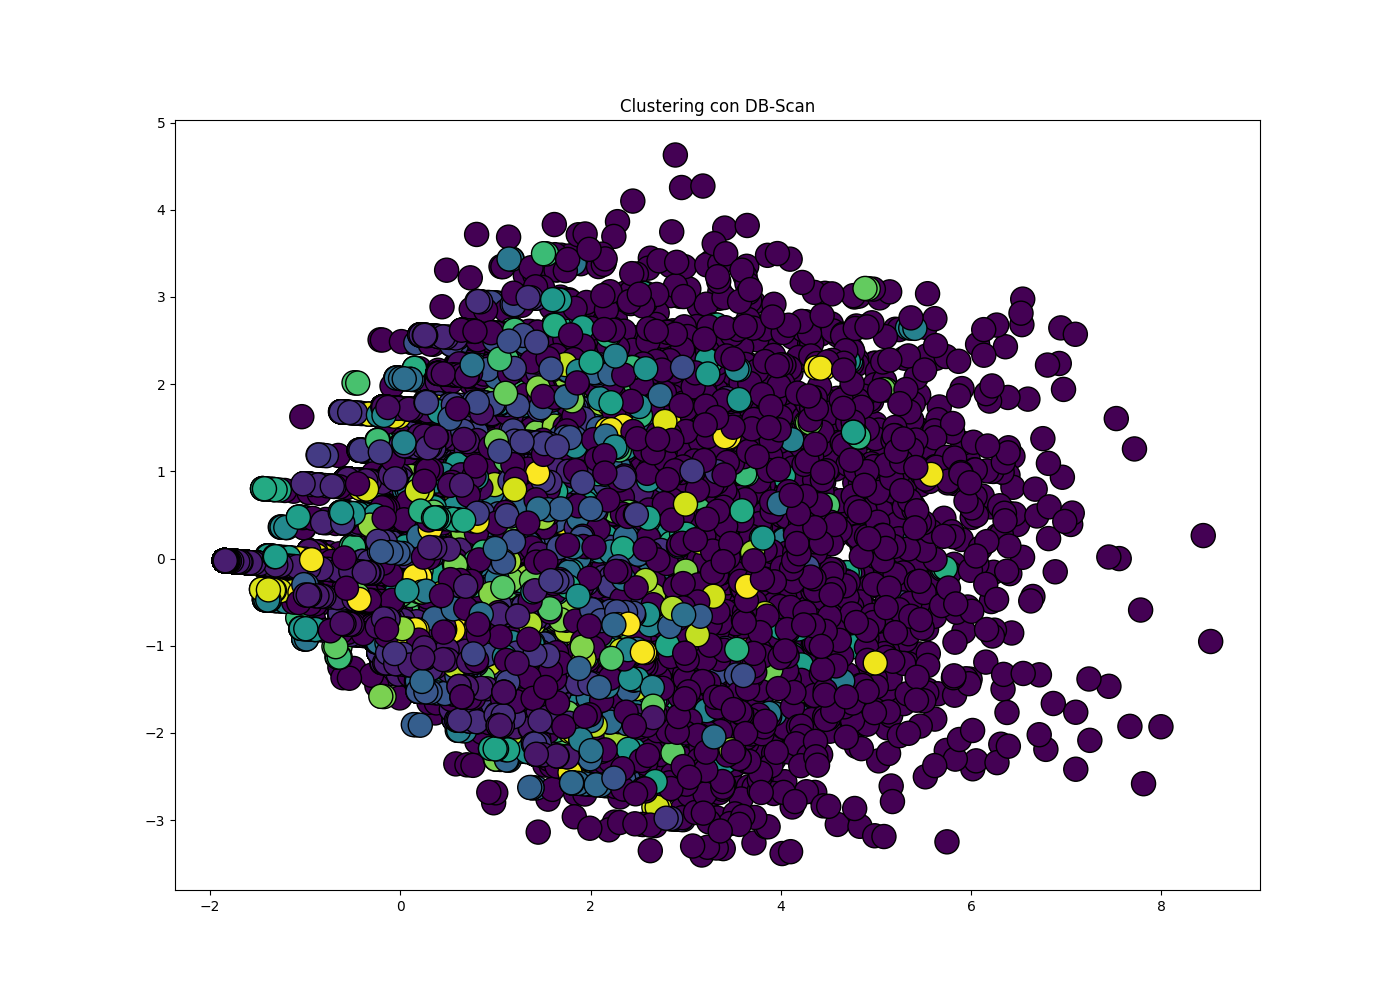
\includegraphics[width=8cm]{modelling/DBScan.png}\\
                \end{center}

                Tutte le considerazioni e valutazioni relative ai valori dei parametri scelti saranno effettuate nella fase successiva
                che è quella di Evaluation.


    \chapter{Evaluation}\label{ch:evaluation}

        \section{K-Means Evaluation}\label{sec:k-means-evaluation}
            \subsection{Elbow point}
                Il primo metodo di valutazione dei risultati di cui si intende usufruire è l'elbow point, con l'ausilio della
                libreria Python \textit{scikit-learn}. Dopo aver caricato i valori presenti nel dataset e inizializzato una nuova
                lista (\textit{inertias[]}), abbiamo provveduto ad eseguire il k-means su un numero crescente di cluster, memorizzando
                ad ogni iterazione il valore di inerzia prodotto.
                Quest'ultimo è una misura della qualità dei cluster generati, in quanto si riferisce alla misura di somiglianza ottenuta
                all'interno dei cluster.
                Più bassa è l'inerzia, più simili sono i punti all'interno di un cluster.
                L'inerzia di un cluster è calcolata come la somma delle distanze quadratiche tra ciascun punto del cluster e il
                centroide del cluster stesso.
                Il punto in cui si osserva una diminuzione significativa dell'inerzia indica il numero ottimale di cluster, ovviamente
                si cerca di scegliere il numero di cluster che massimizzi la differenziazione tra cluster e
                minimizzi l'inerzia all'interno dei cluster stessi.

                Il grafico ottenuto è il seguente:

                \begin{center}
                    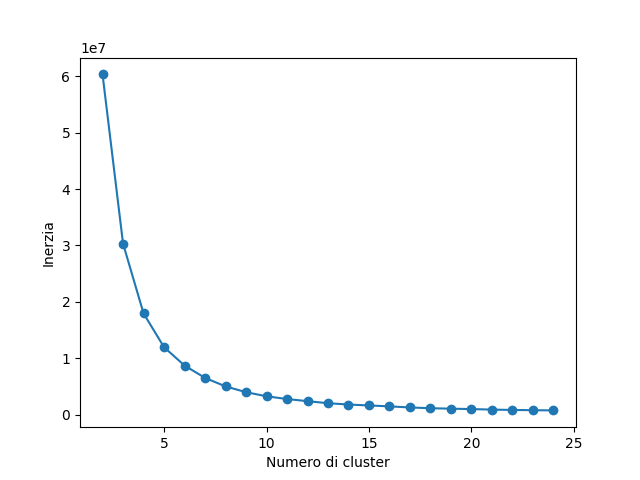
\includegraphics[width=8cm]{evaluation/elbowPoint}\\
                \end{center}

                Come è possibile notare leggendo il grafico, si nota una diminuzione dell'inerzia con l'utilizzo di un k da 7 in su.
                Sebbene l’errore venga minimizzato quando i cluster aumentano, avere un numero eccessivo di cluster implica avere tanti gruppi
                formati da pochi elementi.
                Valutando i grafici ottenuti con l'esecuzione dell'algoritmo k-means al variare della variabile k da 7 a 10 (mostrati di seguito),
                abbiamo notato che, al crescere del valore della variabile k, alcuni cluster si mantengono abbastanza stabili mentre altri
                tendono ad essere fin troppo piccoli. Per questo motivo, risultano migliori i cluster ottenuti con l'utilizzo
                della variabile k pari ad 8 o a 9. Abbiamo ritenuto opportuno demandare tale scelta alla fase successiva, con l'ausilio del calcolo del silhouette
                coefficient.
                \begin{center}
                    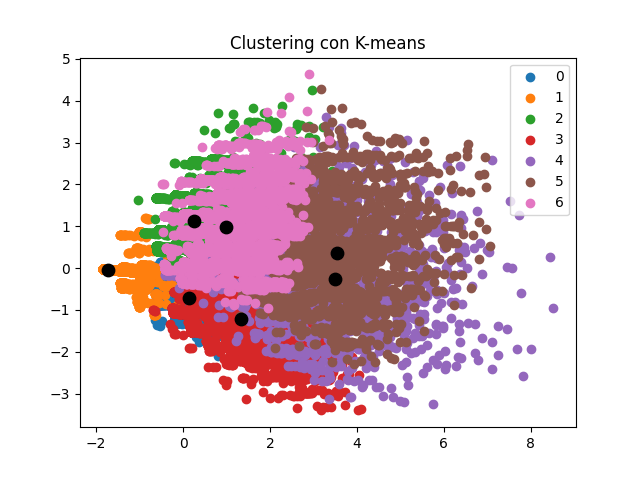
\includegraphics[width=6cm]{evaluation/k=7}
                    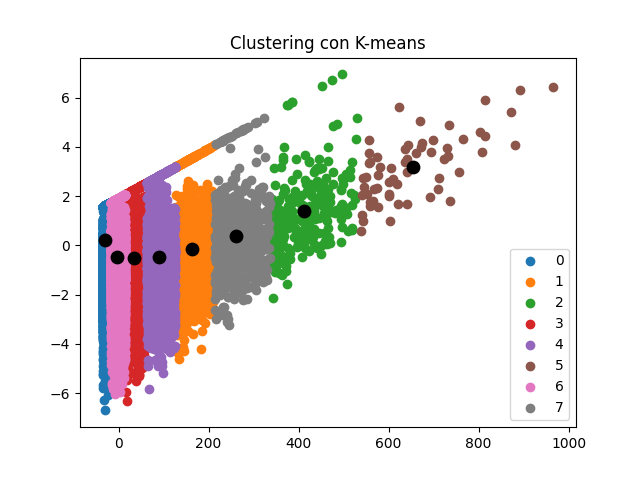
\includegraphics[width=6cm]{evaluation/k=8} \\
                    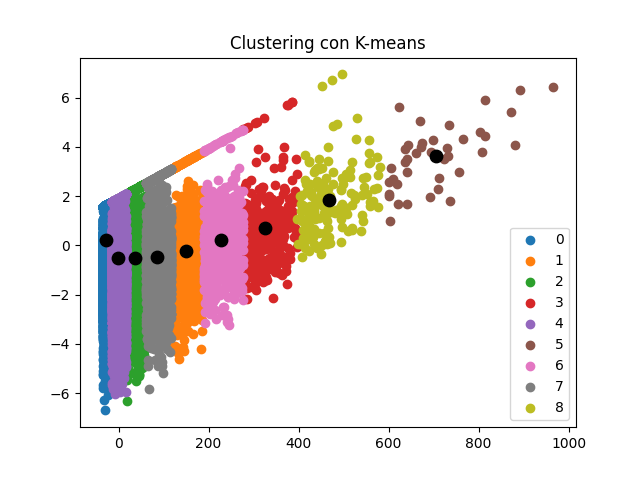
\includegraphics[width=6cm]{evaluation/k=9}
                    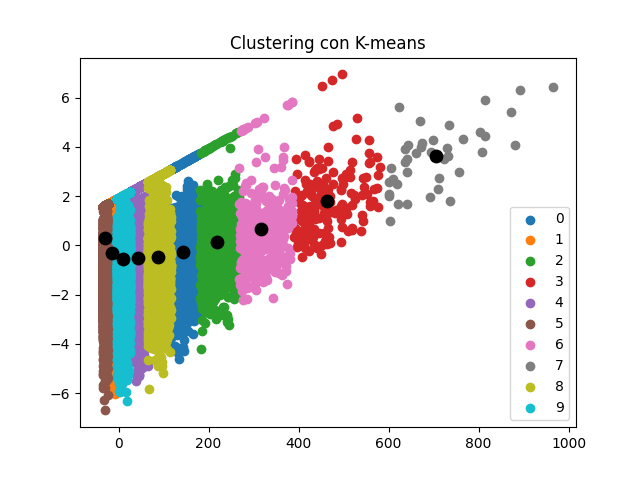
\includegraphics[width=6cm]{evaluation/k=10}
                \end{center}

            \subsection{Silhouette coefficient}
                Un altro metodo di valutazione dei risultati utilizzato è il silhouette coefficient, che permette di calcolare
                quanto i dati siano ben disposti nei cluster generati.
                Dal metodo di valutazione dell'elbow point sopra citato, emerge che il numero di cluster ottimale è un valore
                per k=7 in su.
                Pertanto abbiamo valutato il silhouette coefficient eseguendo il K-Means con un numero di cluster che variava
                nel range da 7 a 10.
                Quindi, utilizzando la libreria di Python sklearn, per ogni valore di 7<=k<=10, abbiamo eseguito il k-means sul
                nostro dataset. Successivamente, tramite la funzione silhouette\_{}score(), abbiamo calcolato il silhouette score,
                ossia una misura della coesione e separazione tra i dati.
                Siamo passati poi a calcolare il silhouette score per ogni campione dei cluster utilizzando l'apposita funzione
                silhouette\_{}samples().

                Vengono riportati di seguito i valori di silhouette score relativi al numero di cluster indicato

                \begin{center}
                    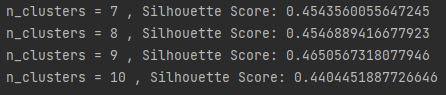
\includegraphics[width=8cm]{evaluation/silhouette score}\\
                \end{center}

                Come mostrato nell'immagine soprastante, il valore di k ottimale è k=9. Quindi, considerando anche le valutazioni
                prodotte con il metodo di Elbow point, il clustering con l'algoritmo k-means è ottimale impostando il parametro
                n\_{}cluster = 9. Questo grafico mostra, per n\_{}cluster=9, il valore del silhouette score e inoltre la divisione
                dei dati nei vari cluster ottenuti.

                \begin{center}
                    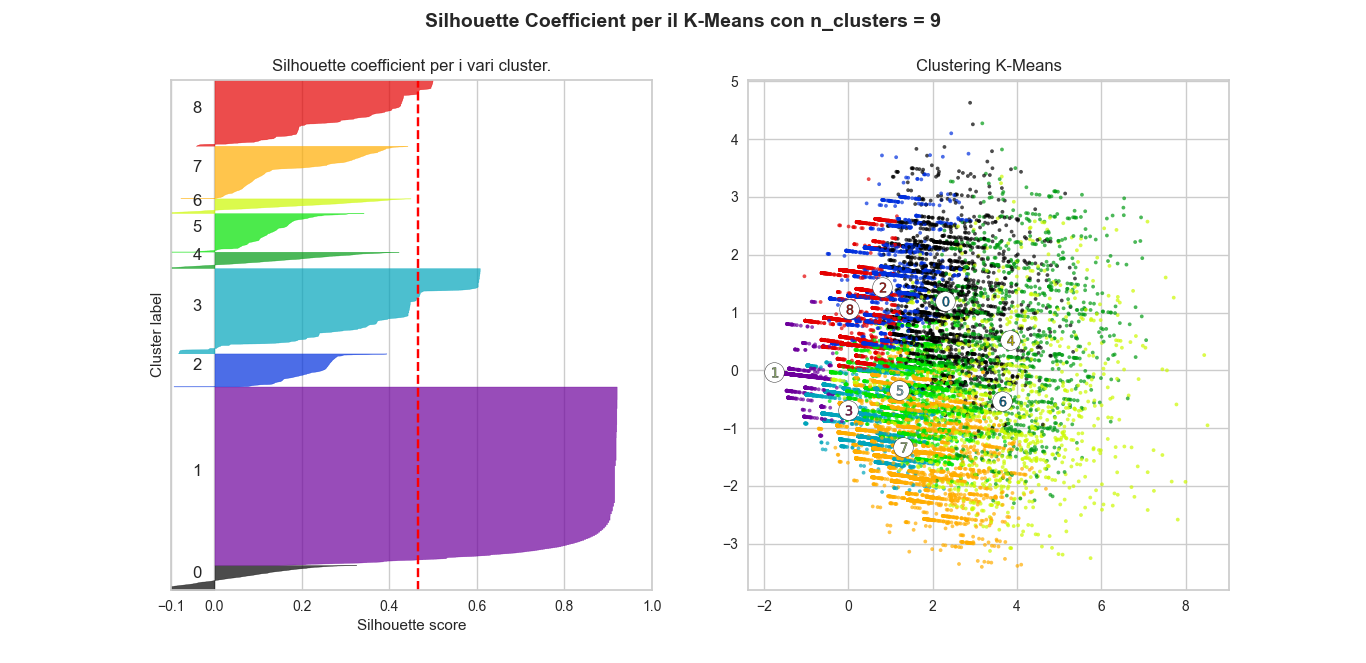
\includegraphics[width=13cm, height=8cm]{evaluation/silhouette_9}\\
                \end{center}


        \section{DB-Scan Evaluation}\label{sec:dbscan-evaluation}
            \subsection{Silhouette Score}
                Il metodo di valutazione, utilizzato per valutare i risultati prodotti dall'algoritmo DB-Scan, è il Silhouette Score
                fornito dalla libreria Python \textit{scikit-learn}. Dopo aver eseguito il DB-Scan con diversi valori sia per l'intorno
                circolare, sia per il minimo numero di punti per considerare un intorno denso, le esecuzioni più rilevanti sono ripostate
                in seguito. I grafici sottoriportati evidenziano il valore del silhouette score e la divisione dei dati nei vari cluster
                ottenuti. La linea verticale tratteggiata è rappresenta la media delle Silhouette Score calcolate in preceneza.

                \begin{center}
                    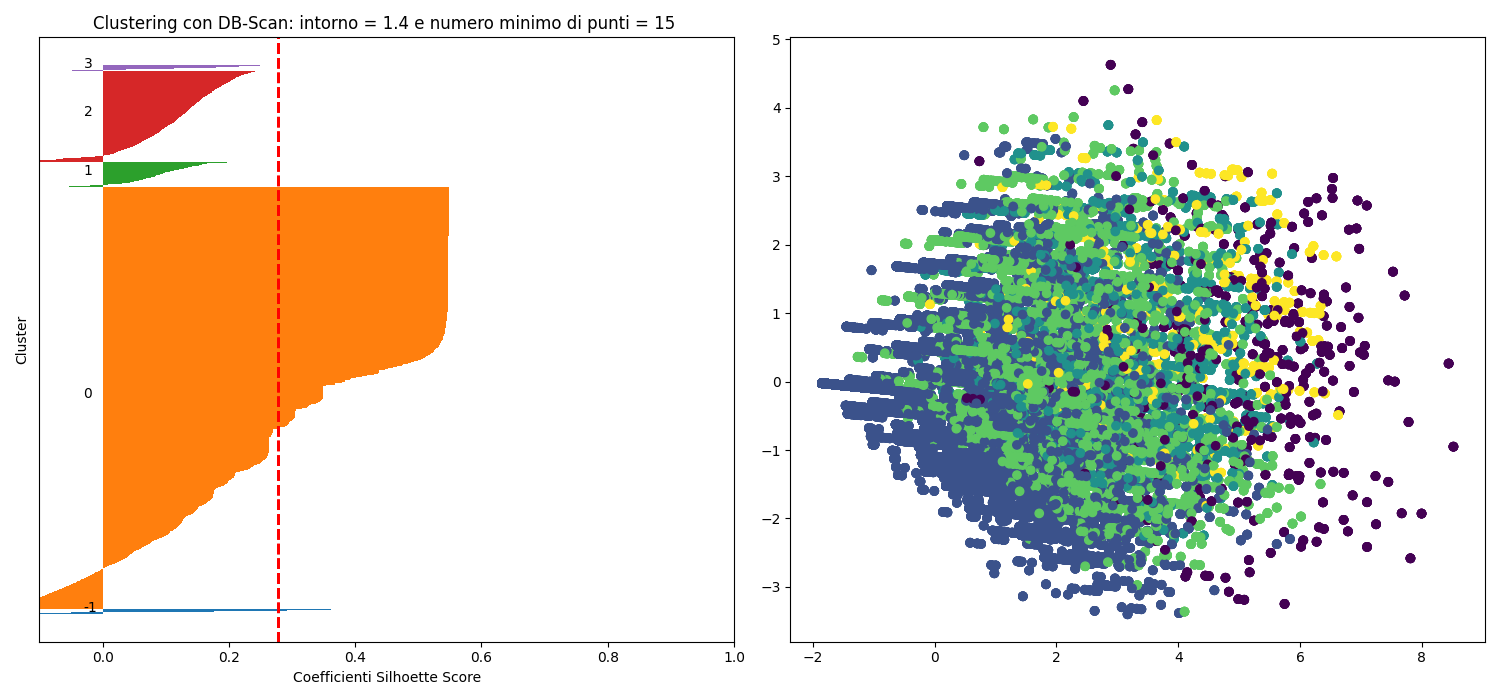
\includegraphics[width=14cm]{evaluation/DBScan_1.4_15.png}
                    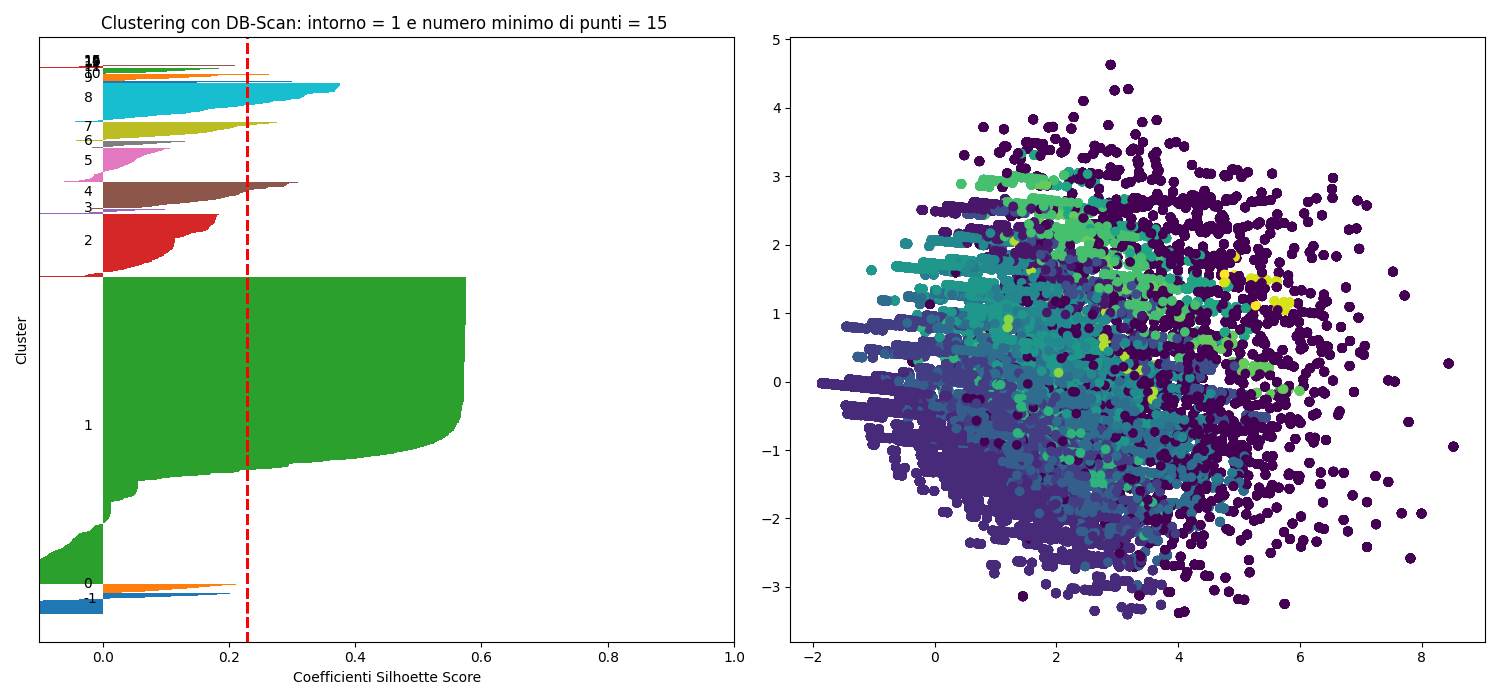
\includegraphics[width=14cm]{evaluation/DBScan_1-15.png} \\
                \end{center}

                Come si può notare nessun grafico risulta essere un clustering ottimale.
                Nel secondo grafico si può notare una suddivisione sub-ottima in quanto:
                \begin{itemize}
                    \item il numero di cluster è maggiore e il cluster contenente più punti ha una dimensione inferiore rispetto al precendente;
                    \item la media delle Silhouette Score è molto simile tra le due;
                    \item la dimensione del cluster (rappresentato dal cluster -1) ha dimensione minore.
                \end{itemize}

                Gli altri risultati, non riportati, hanno gli stessi risultati dei precedenti con una media inferiore e
                una suddivisione non ideale.
                \\Di conseguenza, i valori sub-ottimi sono rappresentati da eps = 1 e min samples = 15.

                \paragraph{}
                Si può notare che l'algoritmo K-Means effettua un clustering migliore, ma il giudizio sul clustering usato sarà offerto dagli
                utenti finali, pertanto la scelta dell'algoritmo migliore tra il K-Means e il DBScan sarà rimandata in fase di utilizzo.
                Questo sarà possibile in quanto il Conversational Agent permetterà ai beta tester di scegliere l'algoritmo di clustering
                da utilizzare, chiedendo direttamente di effettuare tale scelta prima di iniziare il clustering.

    \chapter{Integrazione con il sistema}\label{ch:integrazione-con-il-sistema}
        Dopo aver scelto l'algoritmo di clustering da utilizzare e le conseguenti valutazioni su di esso, va definito come
        integrarlo ed impiegarlo all'interno del nostro sistema software.
        Gli algoritmi adoperati ci consentono di calcolare, a partire dal dataset di film di cui si dispone, un certo numero di cluster
        contenenti film con caratteristiche simili, come visibile anche dai grafici seguenti.

        \begin{center}
            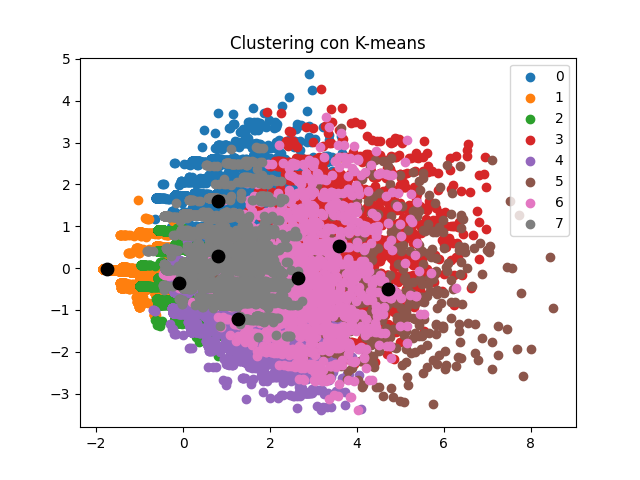
\includegraphics[width=6cm]{modelling/ClusterK-Means}
            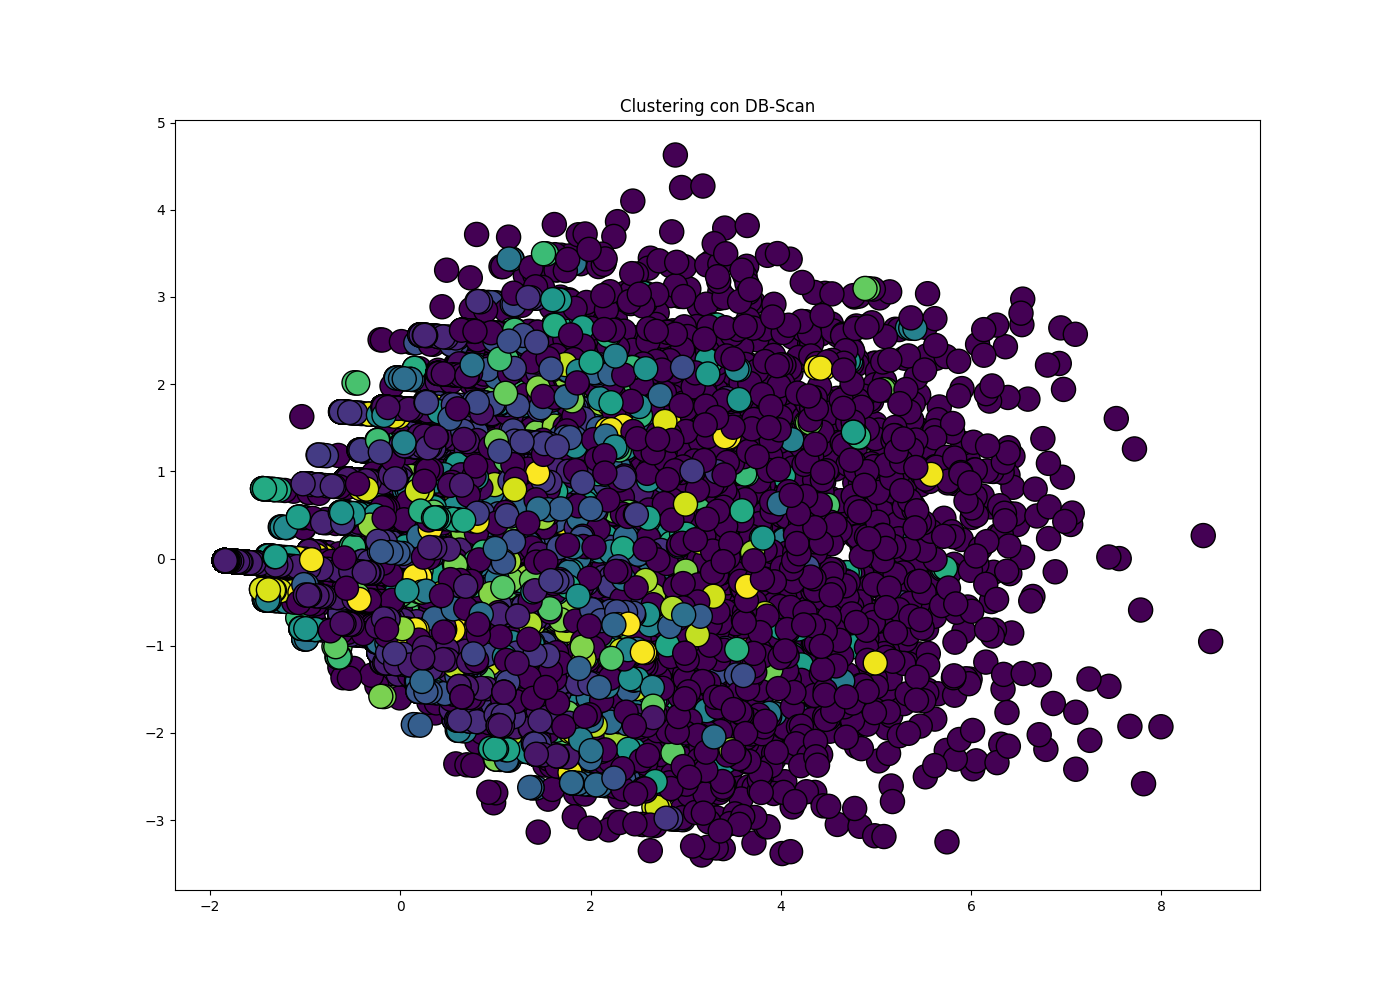
\includegraphics[width=6cm]{modelling/DBScan}
        \end{center}

        \\Una volta ottenuto questo modello, l'obiettivo da raggiungere era partire da una lista di film preferiti di un iscritto
        e consigliarne nuovi che potessero rispecchiare i suoi gusti e le sue preferenze espresse tramite l'applicazione.
        Ad esempio, ipotizziamo che la lista di preferiti dell'utente contenga i seguenti film:
        \begin{itemize}
            \item Storie irlandesi
            \item Diva!
            \item La grande bellezza
            \item Adults in the Room
            \item Ciao amore, vado a combattere
            \item Il piccolo ladro
            \item Polvere di stelle
            \item Home
            \item 120 battiti al minuto
            \item Tutti fratelli nel West... per parte di padre
        \end{itemize}
        Sulla base degli elementi della lista dell'utente, abbiamo costruito un dizionario formato da
        coppie chiave-valore rispettivamente contenenti il titolo e l'anno di un film (chiave) e il cluster di appartenenza (valore).
        Successivamente abbiamo individuato il cluster contenente il maggior numero di elementi della lista di preferiti dell'iscritto
        (\textit{tableCluster}) e salvato all'interno di una nuova lista (\textit{newList}) i film che appartenevano a questa intersezione.
        \begin{center}
            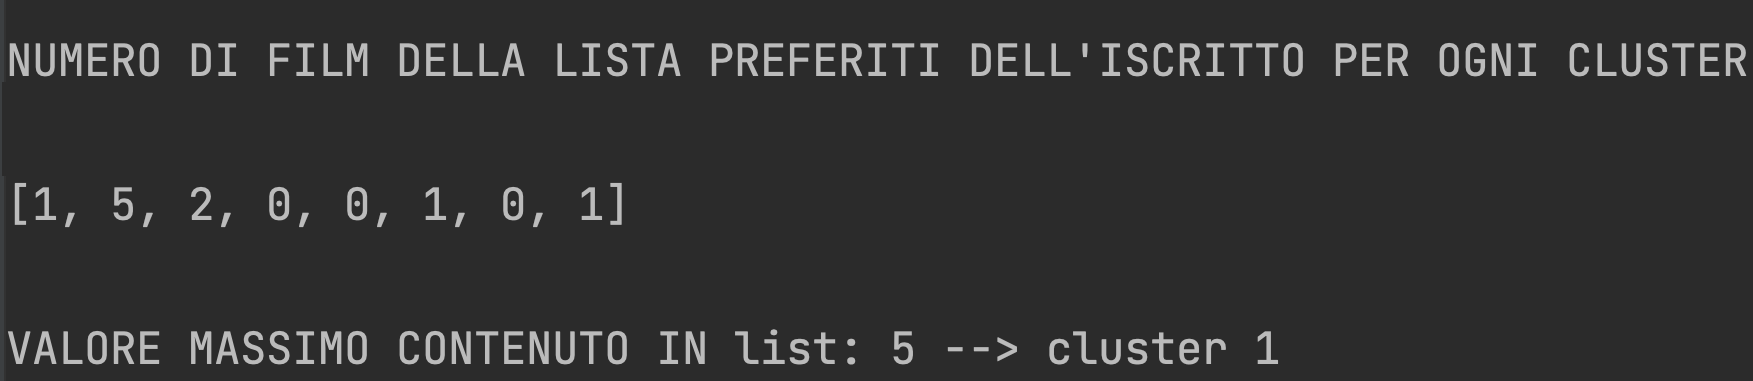
\includegraphics[width=8cm]{modelling/numeroFilmxCluster}\\
        \end{center}

        Abbiamo poi calcolato le distanze metriche medie tra gli elementi di \textit{newList} e tutti i restanti elementi
        del cluster \textit{tableCluster}.
        \begin{center}
            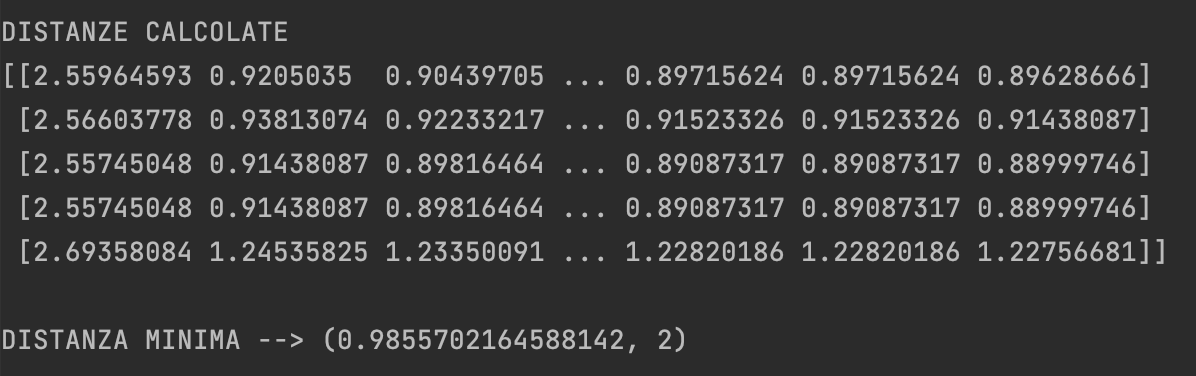
\includegraphics[width=8cm]{modelling/distanzeMetriche}\\
        \end{center}

        Ottenuta questa informazione abbiamo individuato l'elemento con distanza metrica inferiore. Quest'ultimo rappresenta proprio
        il film più vicino alle preferenze espresse dall'utente e quindi il film che verrà consigliato all'iscritto tramite il
        Conversational Agent.
        \begin{center}
            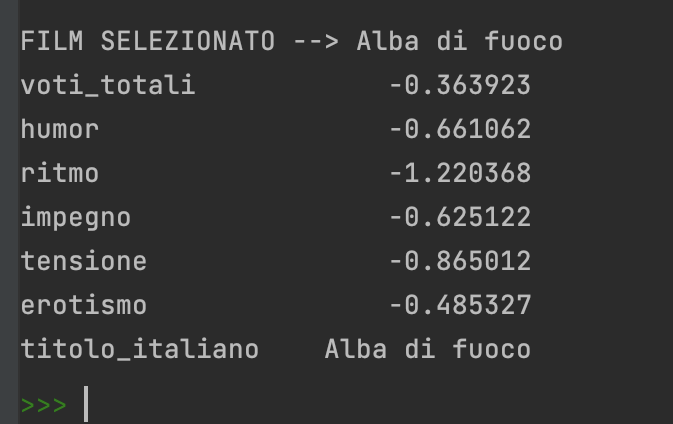
\includegraphics[width=8cm]{modelling/filmSelezionato}\\
        \end{center}

        In merito all'addestramento del Conversational Agent abbiamo usufruito della libreria \textit{Natural Language Toolkit}
        offerta dal linguaggio di programmazione \textit{Python}. Abbiamo inizializzato un array (\textit{pairs}) di coppie domande-risposte,
        in particolare abbiamo ipotizzato una serie di pattern corrispondenti ad espressioni regolari che esprimono statement o domande che
        l'utente può inviare al sistema ed in base ad essi abbiamo definito delle risposte che il nostro CA dovrà fornire all'utente.

        In questo modo andiamo ad istruire il bot su come rispondere alle domande o alle frasi dell'utente. Per diverse domande
        sono state previste risposte multiple, in modo da rendere il bot meno monotono.
        \textit{Pairs} contiene domande e risposte specifiche per la nostra applicazione e per lo scopo
        principale della creazione del bot, ovvero il suggerimento di film in base ai gusti degli iscritti.
        Nel momento in cui l'iscritto digita un messaggio e lo invia, se questo avrà un match con uno dei pattern previsti allora
        verrà visualizzata la risposta appropriata, altrimenti verrà visualizzato un messaggio che invita l'iscritto
        ad esprimere diversamente la sua richiesta.

        Grazie all'utilizzo della libreria \textit{Natural Language Toolkit} i vari passaggi previsti dal Natural Language Processing
        sono eseguiti in automatico e risultano per questo motivo "nascosti".

        Nel caso specifico in cui l'utente richiede un consiglio la risposta verrà data sulla base del risultato della chiamata
        all'algoritmo di clustering per dare un suggerimento mirato, basato sui gusti dell'utente in questione espressi tramite
        l'aggiunta dei film presenti nell'applicazione ad una lista di preferiti.


    \chapter{Deployment}\label{ch:deployment}

        Sarà possibile usufruire del Conversational Agent premendo sull'apposito pulsante 
\includegraphics[width=0.4cm]{deployment/icona_chatbot.png}
        presente nel footer dell'applicazione.
        All'inizio l'utente visualizza un messaggio di benvenuto del bot e successivamente è libero di scrivere le sue
        richieste nell'apposita area visibile in fondo alla schermata. Una volta scritto il messaggio, l'utente dovrà premere il pulsante
        
\includegraphics[width=3cm]{deployment/tasto_invia.png} e dopo pochi secondi la risposta del bot sarà visibile.
        A questo punto sarà possibile inviare un ulteriore messaggio a cui il bot risponderà e così via fino a quando l'utente non deciderà
        di uscire dalla pagina in questione tramite l'apposito pulsante 
\includegraphics[width=3cm]{deployment/tasto_back.png}
        o tramite il tasto  del dispositivo mobile.

        \\Nel caso in cui, l'utente non ha liste a lui associate oppure ha liste ma non
        ha contenuti all'interno delle liste, il Conversational Agent inviterà l'utente a creare ed aggiungere nelle liste i suoi film preferiti.


    \chapter{Glossario}\label{ch:glossario}
        \begin{adjustbox}{width=\columnwidth,center}
            \begin{tabular}{|>{\columncolor{Goldenrod}}c|p{8cm}|}
                \hline \textbf{Conversational Agent/CA} & Bot che interpreta e risponde alle dichiarazioni fatte dagli utenti
                        in un linguaggio naturale, attraverso la  generazione di una conversazione simil-umana.\\
                \hline \textbf{Lista di contenuti} & Sottoinsieme di contenuti offerti da iLike, scelti dagli utenti secondo i loro gusti
                        e inseriti nelle proprie liste disponibili sul proprio profilo personale.\\
                \hline \textbf{Cluster} & Sottoinsieme di contenuti con caratteristiche simili.\\
                \hline \textbf{Machine Learning} & Branca dell'Intelligenza Artificiale che include tutti gli algoritmi
                        che possano imparare dai dati e sulla base di questi fare previsioni.\\
                \hline \textbf{Data Imputation} & Insieme di tecniche che permettono di stimare il valore di dati mancanti
                        sulla base dei dati disponibili oppure mitigare il problema dei dati mancanti.\\
                \hline \textbf{Blox Plot} & Rappresentazione grafica utilizzata per descrivere la distribuzione di un campione
                        tramite la media e deviazione standard.\\
                \hline \textbf{Utente} & Iscritto, cioè persona registrata ad iLike.\\
                \hline
            \end{tabular}
        \end{adjustbox}

\end{document}